% !TEX root = ../../report.tex
\section{Hardwareaufbau}
\begin{Spacing}{\mylinespace}

Die Hardware \\

Beschreibung wie der Tisch gebaut ist\\

\begin{figure}[hbtp]
	\centering
	\label{fig:laboraufbauaufbau}
	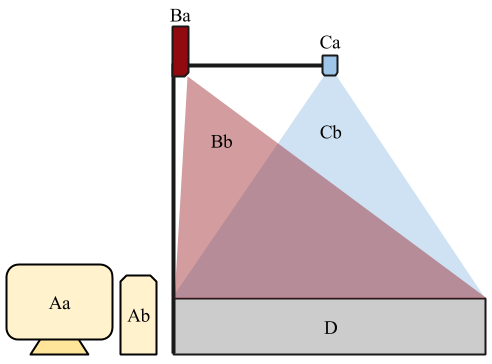
\includegraphics[width=0.8\textwidth]{graphics/Aufbau.png}
	\caption{Laboraufbau}
\end{figure}

\begin{enumerate}  
      \item (A) Steuerrechner
      \begin{enumerate}
         \item Kontrollbildschirm
         \item Rechner
      \end{enumerate}
      \item (B) Projektion
      \begin{enumerate}
         \item Projektor
         \item Projektionsperspektive
      \end{enumerate}
      \item (C) Höhenerfassung
      \begin{enumerate}
         \item Microsoft Kinect
         \item Erfassungsperspektive
      \end{enumerate}
      \item (D) Sandkasten
 \end{enumerate}
   
Was für Rechner dranne hängt\\
Was für Beamer dranne hängt\\
Was das mit dem Sand war\\

\begin{figure}[hbtp]
	\centering
	%Bild oben
	\subfloat[Kinect Hardware]{
	\label{fig:kinHW}
	\inputTikZ{graphics/kinectHW}
	}
	\hfill
	% Bild unten
	\subfloat[Kinect Sichtfeld im Nahmodus]{
	\label{fig:fov}
	\inputTikZ{graphics/fov}
	}
	\caption{Kinect Sensor}
\end{figure}

Die Konstruktion\\
Der Aufbau

\end{Spacing}
\newpage
\clearpage
%% End Of Doc